% Template for ICIP-2019 paper; to be used with:
%          spconf.sty  - ICASSP/ICIP LaTeX style file, and
%          IEEEbib.bst - IEEE bibliography style file.
% --------------------------------------------------------------------------
\documentclass{article}
\usepackage{spconf,amsmath,graphicx}
\usepackage[style=IEEE]{biblatex}
\usepackage{float}
\addbibresource{lib.bib} % note the .bib is required

% Example definitions.
% --------------------
\def\x{{\mathbf x}}
\def\L{{\cal L}} 
% Title.
% ------
\title{Computer Vision Coursework}
%
% Single address.
% ---------------
\name{Alfie Rushby}
\address{}
%
% For example:
% ------------
%\address{School\\
%	Department\\
%	Address}
%
% Two addresses (uncomment and modify for two-address case).
% ----------------------------------------------------------
%\twoauthors
%  {A. Author-one, B. Author-two\sthanks{Thanks to XYZ agency for funding.}}
%	{School A-B\\
%	Department A-B\\
%	Address A-B}
%  {C. Author-three, D. Author-four\sthanks{The fourth author performed the work
%	while at ...}}
%	{School C-D\\
%	Department C-D\\
%	Address C-D}
%
\begin{document}
%\ninept
%
\maketitle
%
\begin{abstract}
The abstract should appear at the top of the left-hand column of text, about
0.5 inch (12 mm) below the title area and no more than 3.125 inches (80 mm) in
length.  Leave a 0.5 inch (12 mm) space between the end of the abstract and the
beginning of the main text.  The abstract should contain about 100 to 150
words, and should be identical to the abstract text submitted electronically
along with the paper cover sheet.  All manuscripts must be in English, printed
in black ink.
\end{abstract}
%
\begin{keywords}
One, two, three, four, five
\end{keywords}
%
\section{Introduction}
\label{sec:intro}

This paper focuses on the aspect of two attempts to segment flowers in a small dataset called Oxford Flower Dataset \autocite{nilsbackVisualVocabularyFlower2006}. The specific dataset is of around 750 flowers, with various species, where the images themselves each contain one flower. The difficulty, then, is to create a consistent solution to segmenting these flowers with the background. These flowers have varying viewpoints, colours, lighting, posing, shape, etc, and so the act of 'knowing' what a flower is with so much variance is very difficult.
\section{Literature Review}
\label{sec:format}

This specific dataset has seen classical attempts at segmenting the flowers. The method uses an approximate segmentation with learned distributions for the background and foreground, and then it iterates on improving the foreground segmentation through using a geometric model of what a flower should look like, until it can converge onto some flower segmentation \autocite{nilsbackDelvingDeeperWhorl2010}. This specific method achieved its performance through a rudimentary learning method, which is by using a set of sample images to create a 'learned' distributions. 

The method is affine invariant, but is still susceptible to colour/lighting variations. To circumvent this, a deep learning approach can be used to expand on the early uses of learning from data, specifically a U-net \autocite{ronnebergerUNetConvolutionalNetworks2015}. This expands on the principle by iteratively learning a set of filters that extract progressively more abstract features as you go down the first half of the network with lowering spatial information. The idea then is that these features would only encode the flower and background, or something useful to then be upscaled with another set of filters into an output segmentation, specifically up-convolutions.

This method removes the need for any assumptions on how a flower is structured, as the entire 'structure' and the concept of a 'flower' is learnt in the fast half. The only downside with this method is its dependence on data, where the quality and quantity of this data affects the performance to a great extent. 

Another method, SegNet \autocite{badrinarayananSegNetDeepConvolutional2017}, exists, with the main differentiator being that it doesn't use convolutions to upscale directly, and uses pooling indexes to help with the upsampling. This isn't as popular as U-Net because it isn't as direct in learning the upscaling sequence with convolutions. 

All of these methods requires data, and the learning of the first section, the downsampling that lowers the spatial resolution progressively, is the same as any classification CNN, like AlexNet or ResNet \autocite{krizhevskyImageNetClassificationDeep2012,heDeepResidualLearning2016}. Training these networks often uses methods like Batch Normalisation, which prevents neuron outputs from spiralling into massive values \autocite{ioffeBatchNormalizationAccelerating2015}, and Dropout, which make the network more robust and lessen overfitting by disabling parts of the network during training \autocite{srivastavaDropoutSimpleWay2014}. 

Smaller dataset training in particular has popular configurations for maximizing training efficiency. Along with what has been spoken of, Data Augmentation is another method to expand the dataset by applying affine transformations, along with possible colour variations. This has been shown to reduce overfitting \autocite{shortenSurveyImageData2019} by increasing the model's generalization (through a larger dataset).

These methods can be used together in specific ways to maximize the usefulness in small dataset applications, where the additional concept of injecting this data augmentation technique in the middle of training can maximize its effectiveness \autocite{thanapolReducingOverfittingImproving2020}. 

It is also possible to transfer learn, or fine tune pre-trained models to use their more general convolutions as a boost in training, where a pre-trained set of weights for the down-convolution can help it lock into a useful area of search on the onset. It has been shown that pre-training helps with generalizing performance by finding a better 'minima' in loss \autocite{pmlr-v9-erhan10a}.


\section{Methodology}


\subsubsection{Data pre-processing}

The dataset by default has more than 2 labels for the segmentation, and has a number of flowers that are unlabelled. The labels themselves include more than 2 classes at times, and so some labels need to be merged with the flower and background class.

First, the flowers without labels are deleted, resulting in 846 labelled flower images to work with. The possible classes for the labelled pixels are null, flower, background, leaves, and sky. Null and flower are often just the inner flower and its boundary, and so can be combined. The other labels are all 'background' and so can also be combined into the background class. This has been directly applied to the dataset with MATLAB and saved so that it doesn't need to be re-applied on every run of training.

For the transfer learning method, it is also important to note that the images and labels will be resized to 224x224 to fit the ResNet input dimension. This is done with MATLAB's resize algorithm.

The images of the flowers are also noisy due to the resizing algorithm used, and so a minor blur has been applied to smooth out the artefacts. 

\begin{figure}[H]
    \centering
    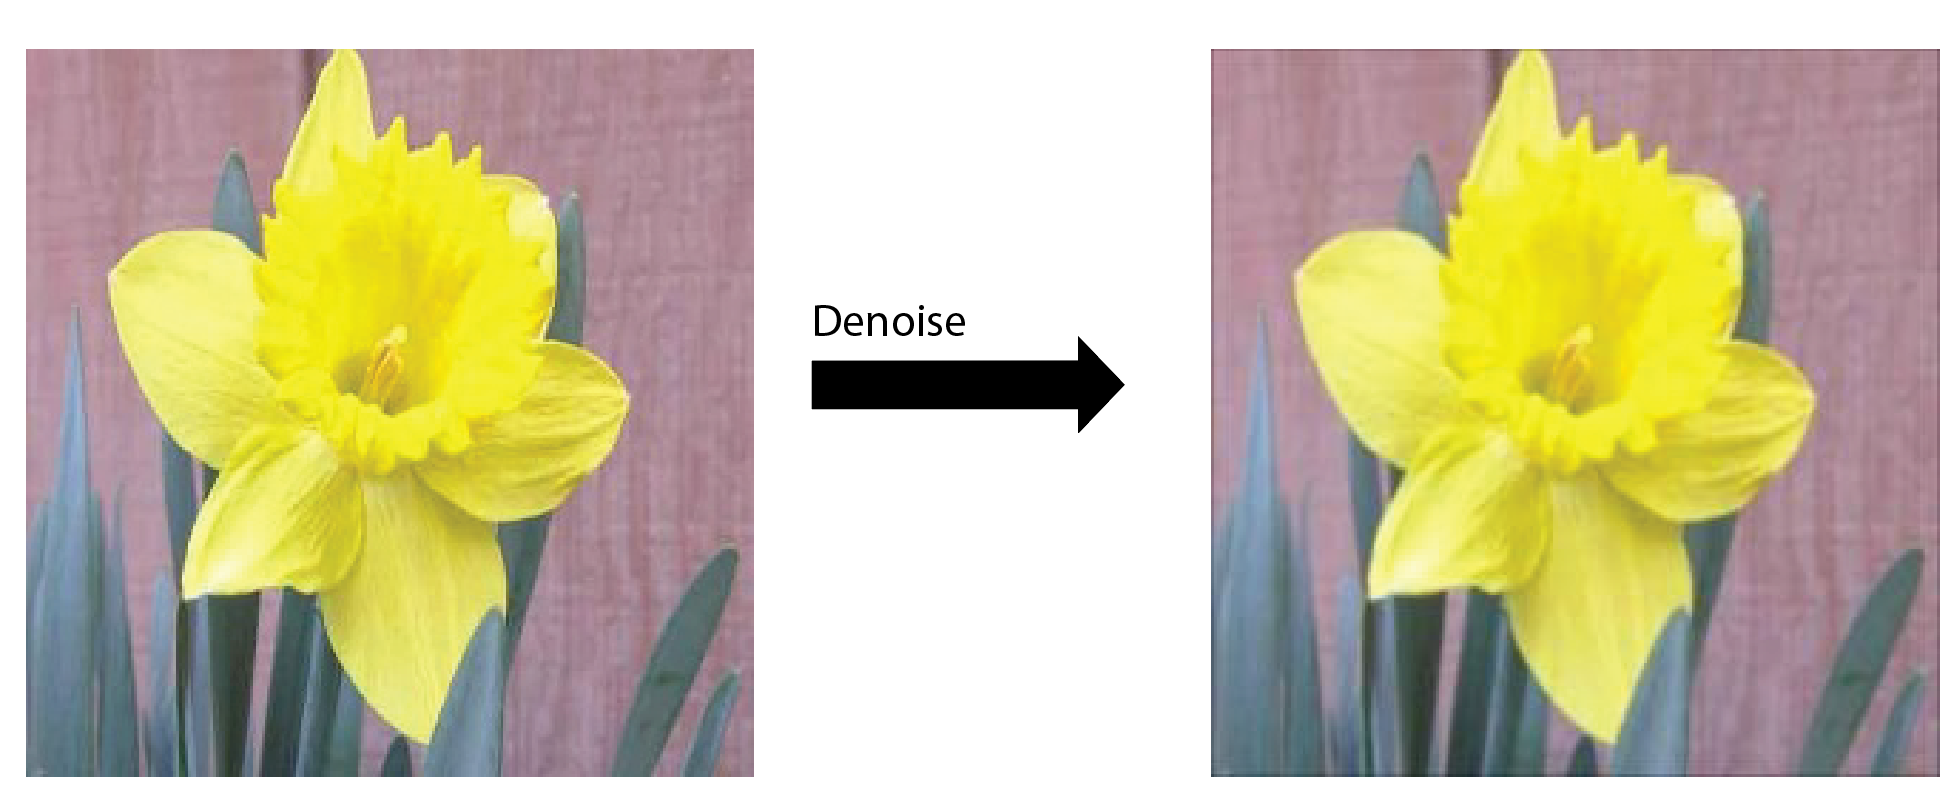
\includegraphics[width=\linewidth]{denoise.png}
    \caption{Denoising of an image in the dataset}
    \label{fig:enter-label}
\end{figure}

This method does add a blur to the image, but it smooths out the artefacts which seems to favour the training if you look at the \textbf{Evaluation} section.

\subsubsection{Data Augmentation}

Along with pre-processing, an active data augmentation method has been utilized during training, where a set of random affine transformations are applied to the images. This includes X and Y translations between -10 and 10 pixels, an X reflection, and a random scaling factor between 1 to 1.5.

\subsubsection{Segmentation with a 'from scratch' model}

From what has been discussed in the literature review, a U-Net along with Batch Normalization and Dropout has been chosen:

\begin{figure}[H]
    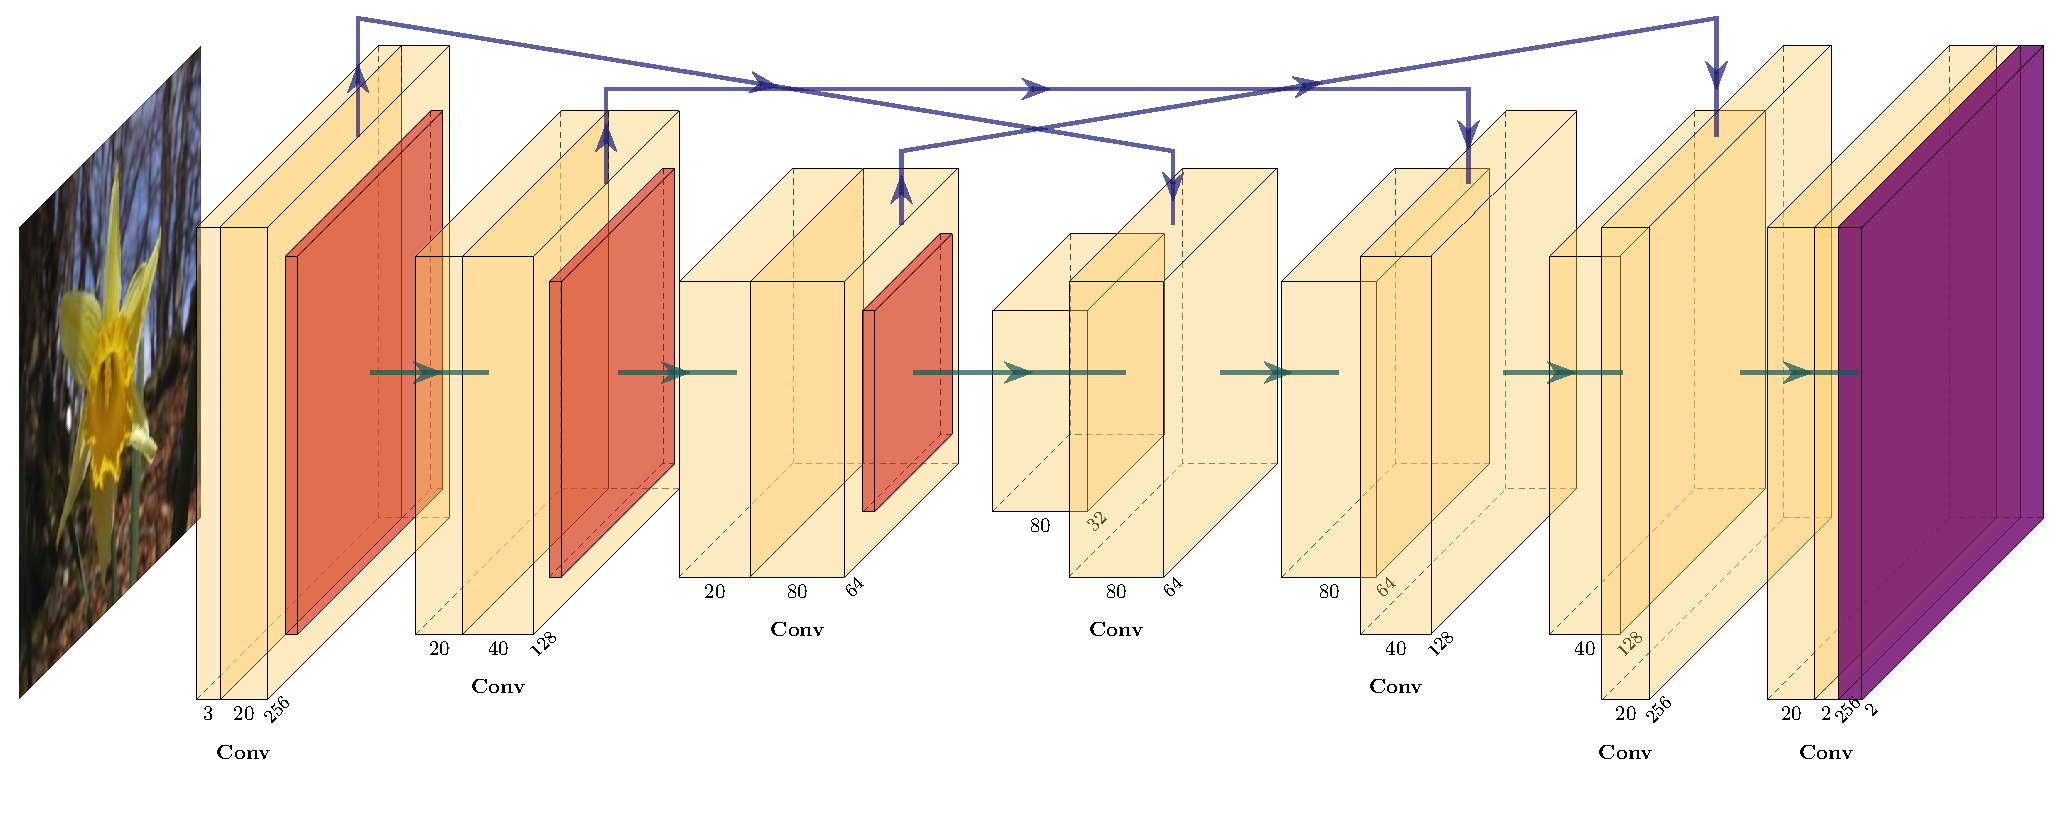
\includegraphics[width=\linewidth]{unet.pdf}
    \caption{Model Architecture}
\end{figure}

Relu and batch-normalization layers have been left out of the diagram to save space, but you can assume that every up-convolution has a batch-normalization and every convolution has a ReLu layer. 

The network was trained with a maximum epoch of 256, with a linear learning rate of 0.001 with the 'Stochastic Gradient Descent with momentum' optimizer. The simple method was chosen so that a focus could be put on the architecture, as there was not a need for optimizing the time taken to train for such a small model.

\begin{figure}[H]
    \centering
    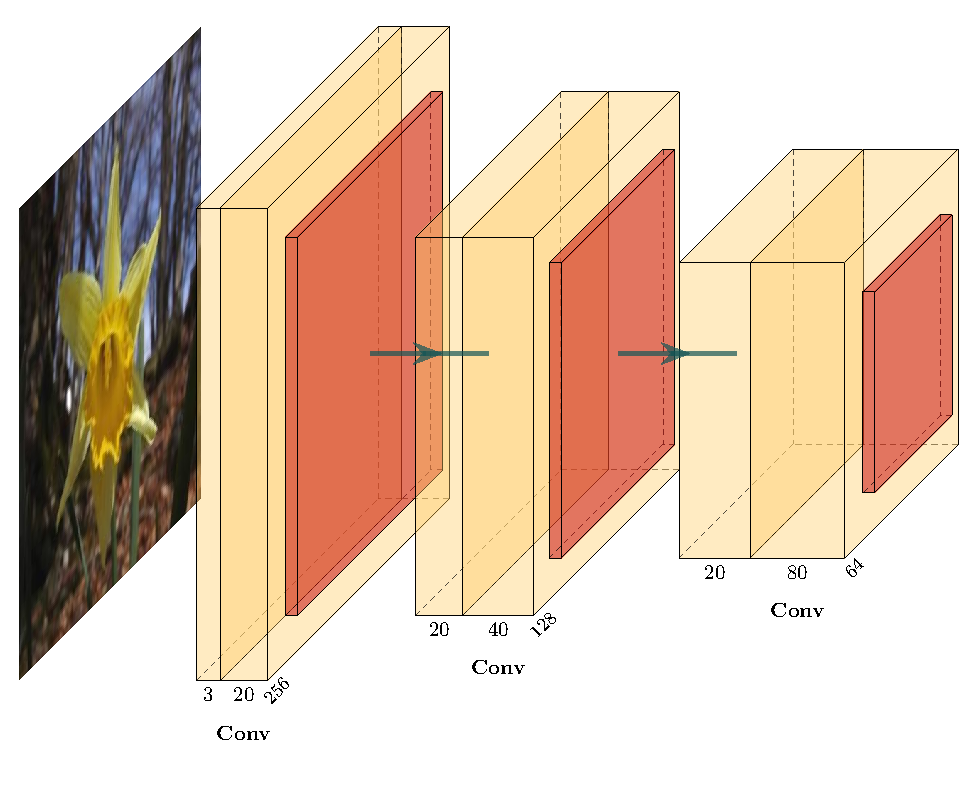
\includegraphics[width=\linewidth]{unetEncode.pdf}
    \caption{Encoder Architecture}
\end{figure}

The encoder has been set up to start by creating 20 filters from the first convolution, without decreasing the spatial resolution. From this, it follows the pattern of doubling the filters and halving the resolution to 32x32 pixels. 

No more layers were added as it added complexity and made training difficult. It uses 3x3 filters all the way through, with the lowering spatial resolution negating the need for larger ones.

\begin{figure}[H]
    \centering
    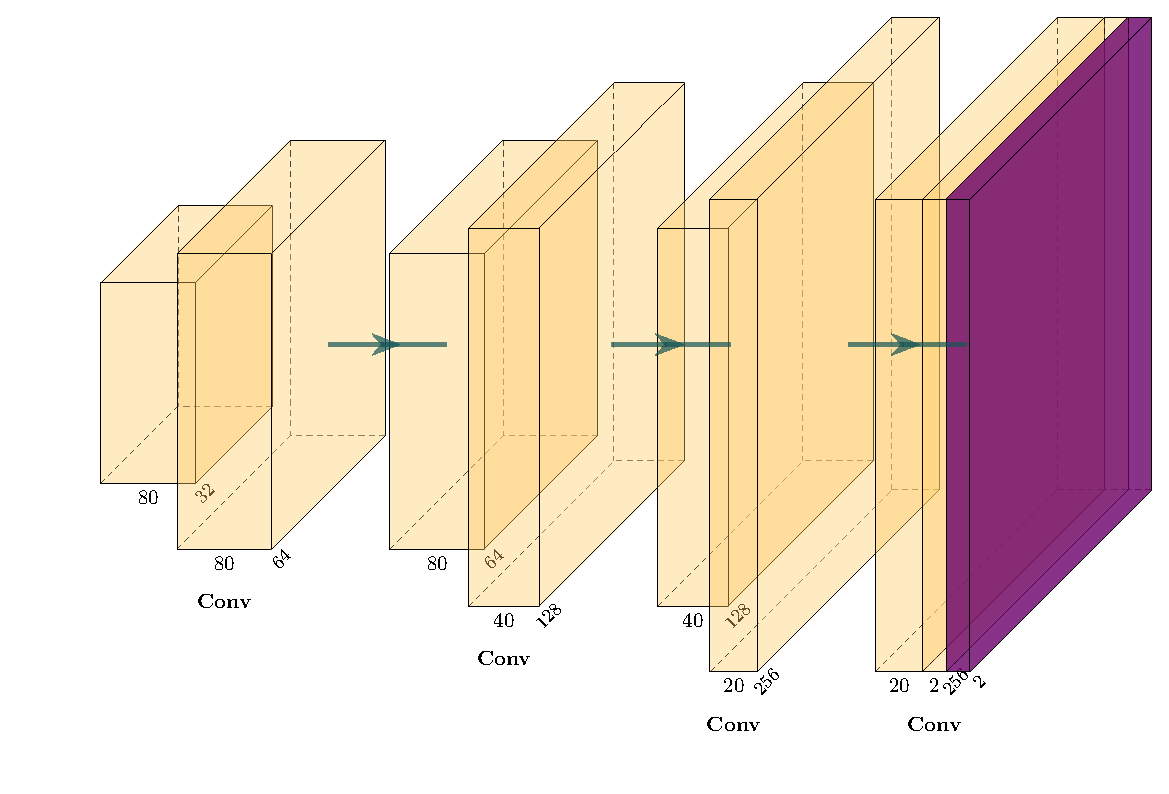
\includegraphics[width=\linewidth]{unetDecode.pdf}
    \caption{Decoder Architecture}
\end{figure}

The decoder works similarly, except that it uses convolutions to upscale, not max-pooling. The end layer is a softmax layer. It uses 4x4 filters.

\subsubsection{Segmentation with a 'Pre-trained' model}

Resnet-18 was used as the base to pre-train off of. This was chosen because it is a relatively small classifier trained on a 1000 class image dataset. It is hypothesized that the first few layers are useful from this to fine tune towards the flower segmentation problem. 

\begin{figure}[H]
    \centering
    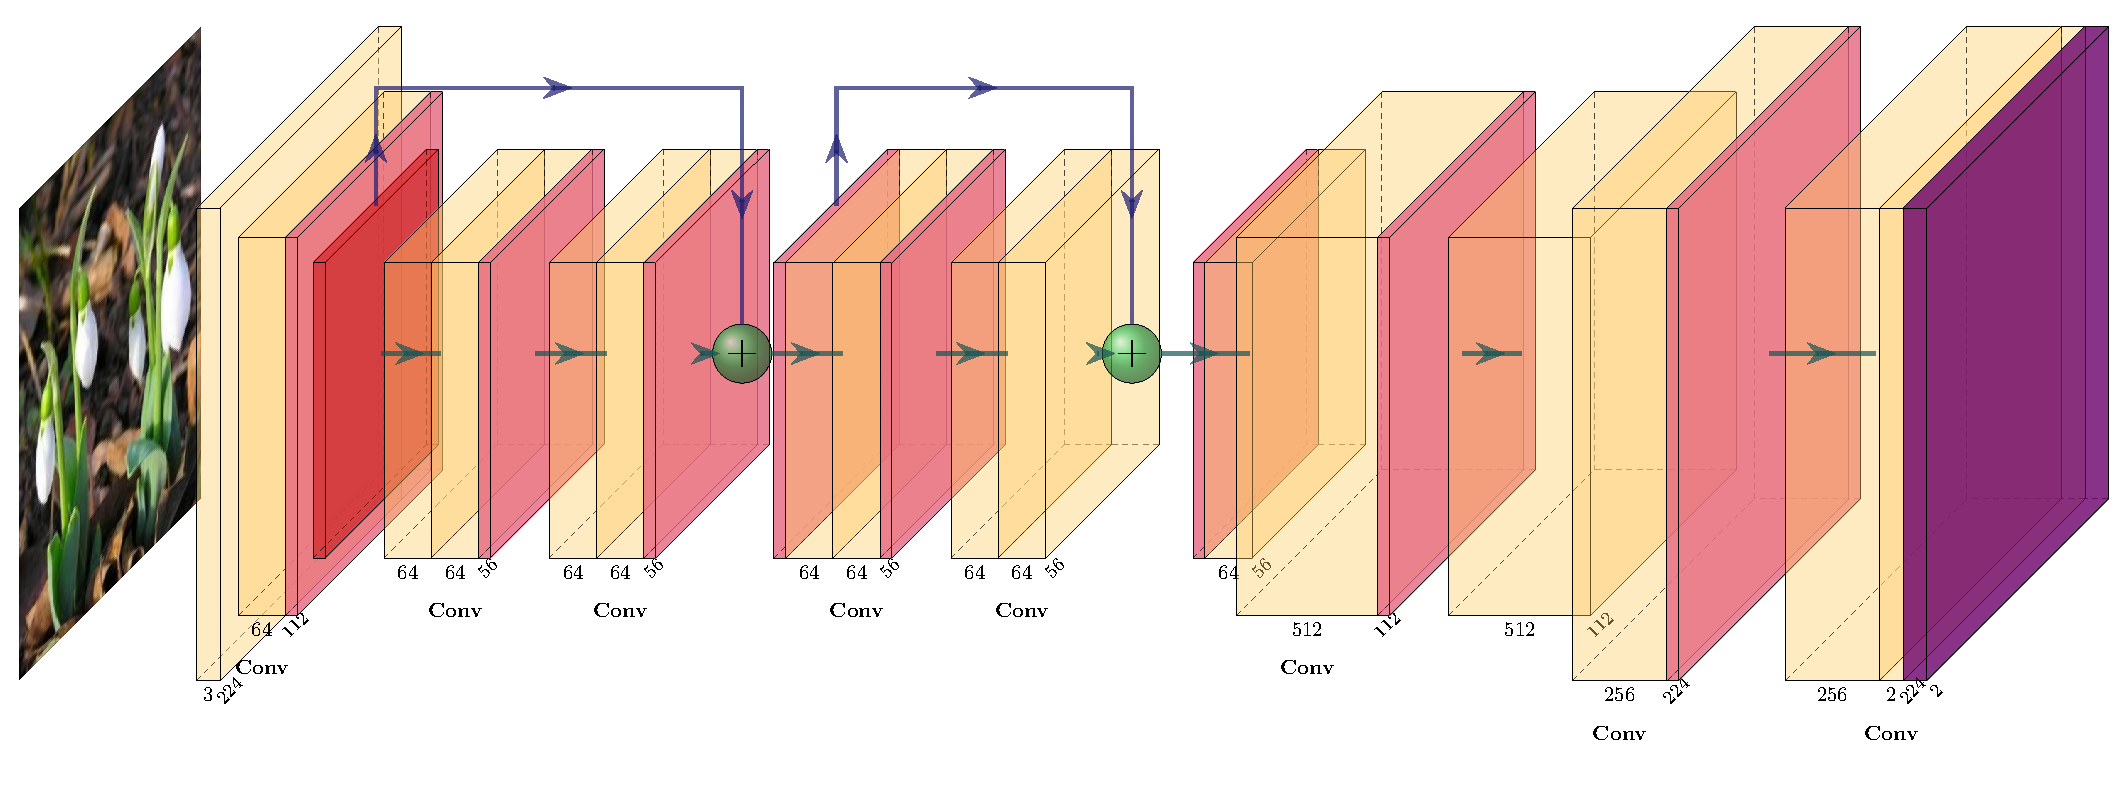
\includegraphics[width=\linewidth]{resnetUnet.pdf}
    \caption{ResNet + U-Net Model Architecture}
\end{figure}

As ResNet is a classifier a number of modifications were done to make it segment images. A number of the resNet convolutions were removed to make training easier, leaving just two sets of branched 'layers'. The pink layers are ReLu layers as they hold a more important role here, so they are included. Batch Normalization is not shown, but appears after every convolution in the downsample area.

An interesting quirk from this is that there is only one pooling of downsampling, which is at the start. This is due to removing the ResNet layers past the 2 pairs. Such a quirk doesn't seem to negatively impact performance.

\begin{figure}[H]
    \centering
    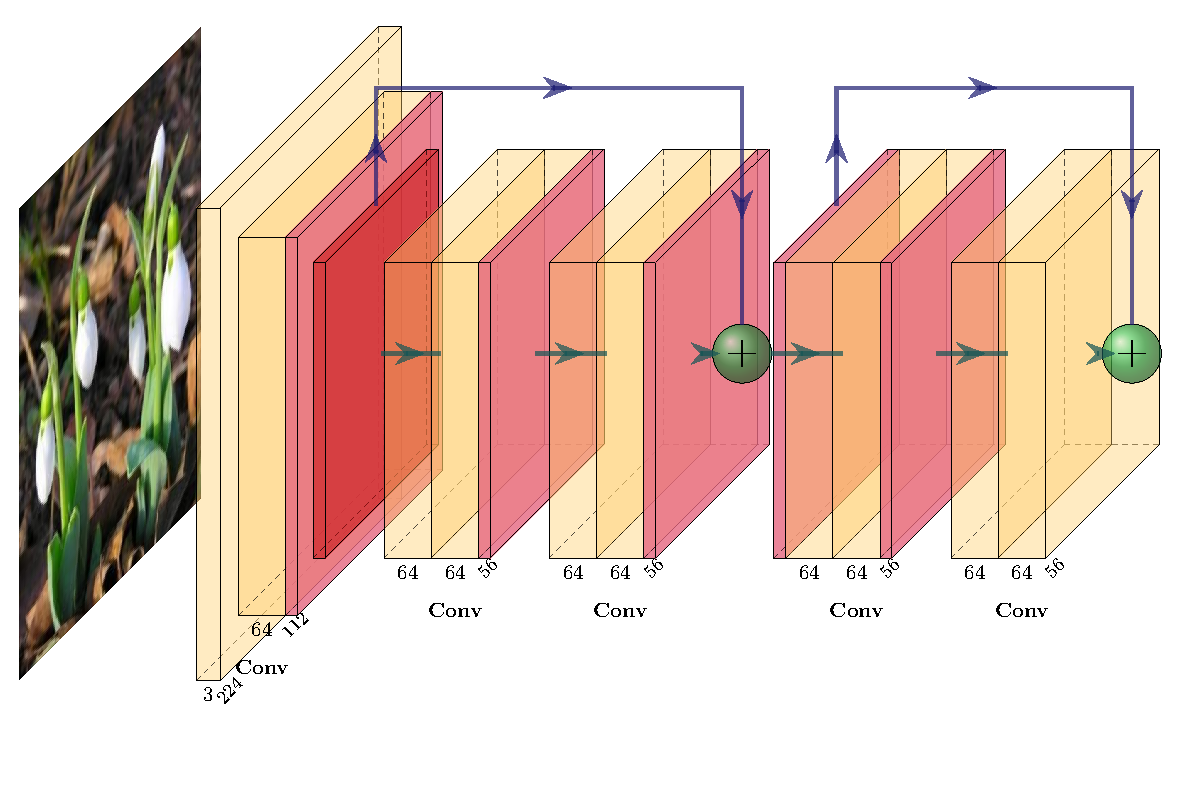
\includegraphics[width=\linewidth]{resnetUnetEncode.pdf}
    \caption{Encoder Architecture}
\end{figure} 

There are two skip connections that sum the previous convolution outputs, where it is done in pairs. This part is taken from ResNet-18 and is pre-trained.

When training, the learning rate of these layers was set to 0.4. Instead of stopping learning completely, a smaller learning rate will allow the training to adapt the first layers, and with the fact that they are already trained from another dataset, gain an advantage when learning.

\begin{figure}[H]
    \centering
    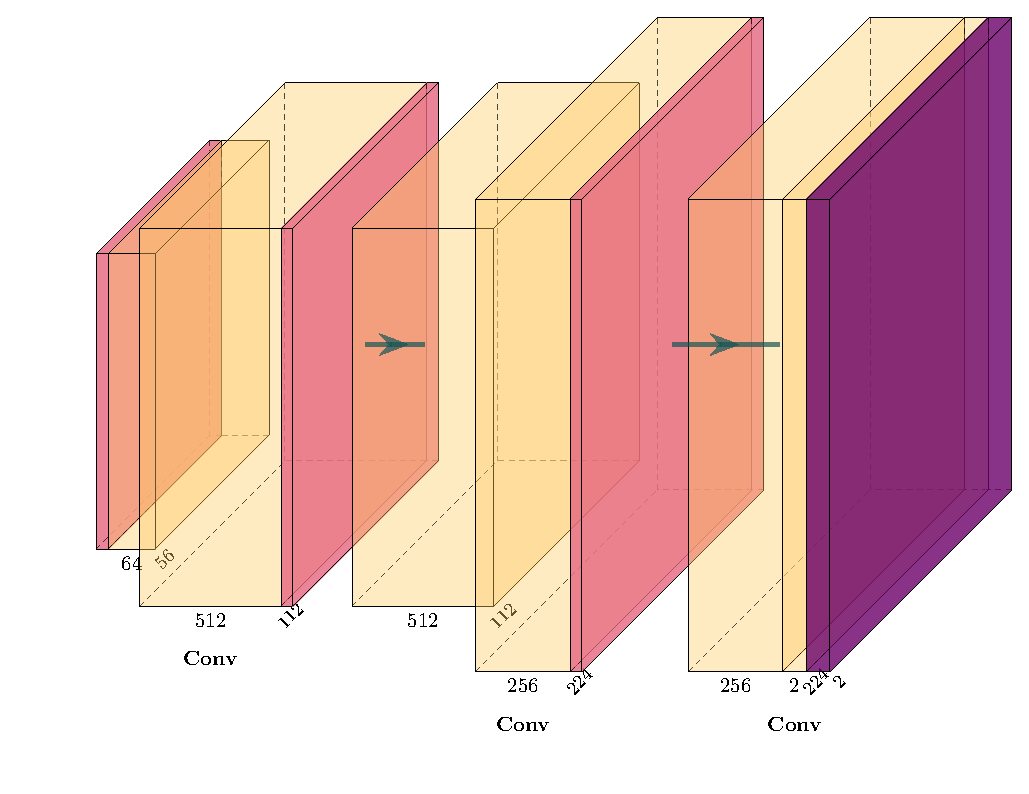
\includegraphics[width=\linewidth]{resnetUnetDecode.pdf}
    \caption{Decoder Architecture}
\end{figure} 

The decoder follows a similar structure to the U-Net used in the 'from-scratch' model. The main difference is there is one less convolution pass, as the dimension inputted to it only requires 2 2x2 filter passes on up-convolutions, from 56x56 to 224x224. The filter sizes were chosen to accommodate the input dimension.

\section{Evaluation}
\label{sec:majhead}

Major headings, for example, "1. Introduction", should appear in all capital
letters, bold face if possible, centered in the column, with one blank line
before, and one blank line after. Use a period (".") after the heading number,
not a colon.

\subsection{Subheadings}
\label{ssec:subhead}

Subheadings should appear in lower case (initial word capitalized) in
boldface.  They should start at the left margin on a separate line.
 
\subsubsection{Sub-subheadings}
\label{sssec:subsubhead}

Sub-subheadings, as in this paragraph, are discouraged. However, if you
must use them, they should appear in lower case (initial word
capitalized) and start at the left margin on a separate line, with paragraph
text beginning on the following line.  They should be in italics.

\section{PRINTING YOUR PAPER}
\label{sec:print}

Print your properly formatted text on high-quality, 8.5 x 11-inch white printer
paper. A4 paper is also acceptable, but please leave the extra 0.5 inch (12 mm)
empty at the BOTTOM of the page and follow the top and left margins as
specified.  If the last page of your paper is only partially filled, arrange
the columns so that they are evenly balanced if possible, rather than having
one long column.

In LaTeX, to start a new column (but not a new page) and help balance the
last-page column lengths, you can use the command ``$\backslash$pagebreak'' as
demonstrated on this page (see the LaTeX source below).

\section{PAGE NUMBERING}
\label{sec:page}

Please do {\bf not} paginate your paper.  Page numbers, session numbers, and
conference identification will be inserted when the paper is included in the
proceedings.

\section{ILLUSTRATIONS, GRAPHS, AND PHOTOGRAPHS}
\label{sec:illust}

Illustrations must appear within the designated margins.  They may span the two
columns.  If possible, position illustrations at the top of columns, rather
than in the middle or at the bottom.  Caption and number every illustration.
All halftone illustrations must be clear black and white prints.  Colors may be
used, but they should be selected so as to be readable when printed on a
black-only printer.

Since there are many ways, often incompatible, of including images (e.g., with
experimental results) in a LaTeX document, below is an example of how to do
this \cite{Lamp86}.

\section{FOOTNOTES}
\label{sec:foot}

Use footnotes sparingly (or not at all!) and place them at the bottom of the
column on the page on which they are referenced. Use Times 9-point type,
single-spaced. To help your readers, avoid using footnotes altogether and
include necessary peripheral observations in the text (within parentheses, if
you prefer, as in this sentence).

% Below is an example of how to insert images. Delete the ``\vspace'' line,
% uncomment the preceding line ``\centerline...'' and replace ``imageX.ps''
% with a suitable PostScript file name.
% -------------------------------------------------------------------------
\begin{figure}[htb]


%
\caption{Example of placing a figure with experimental results.}
\label{fig:res}
%
\end{figure}


% To start a new column (but not a new page) and help balance the last-page
% column length use \vfill\pagebreak.
% -------------------------------------------------------------------------
%\vfill
%\pagebreak

\section{COPYRIGHT FORMS}
\label{sec:copyright}

You must include your fully completed, signed IEEE copyright release form when
form when you submit your paper. We {\bf must} have this form before your paper
can be published in the proceedings.

\section{REFERENCES}
\label{sec:ref}

List and number all bibliographical references at the end of the
paper. The references can be numbered in alphabetic order or in
order of appearance in the document. When referring to them in
the text, type the corresponding reference number in square
brackets as shown at the end of this sentence \cite{C2}. An
additional final page (the fifth page, in most cases) is
allowed, but must contain only references to the prior
literature.

% References should be produced using the bibtex program from suitable
% BiBTeX files (here: strings, refs, manuals). The IEEEbib.bst bibliography
% style file from IEEE produces unsorted bibliography list.
% -------------------------------------------------------------------------
\printbibliography[heading=none]

\end{document}
